\documentclass[journal,12pt,twocolumn]{IEEEtran}

\usepackage{setspace}
\usepackage{gensymb}

\singlespacing


\usepackage[cmex10]{amsmath}

\usepackage{amsthm}

\usepackage{mathrsfs}
\usepackage{txfonts}
\usepackage{stfloats}
\usepackage{bm}
\usepackage{cite}
\usepackage{cases}
\usepackage{subfig}

\usepackage{longtable}
\usepackage{multirow}

\usepackage{enumitem}
\usepackage{mathtools}
\usepackage{steinmetz}
\usepackage{tikz}
\usepackage{circuitikz}
\usepackage{verbatim}
\usepackage{tfrupee}
\usepackage[breaklinks=true]{hyperref}
\usepackage{graphicx}
\usepackage{tkz-euclide}
\usepackage{float}


\usetikzlibrary{calc,math}
\usepackage{listings}
    \usepackage{color}                                            %%
    \usepackage{array}                                            %%
    \usepackage{longtable}                                        %%
    \usepackage{calc}                                             %%
    \usepackage{multirow}                                         %%
    \usepackage{hhline}                                           %%
    \usepackage{ifthen}                                           %%
    \usepackage{lscape}     
\usepackage{multicol}
\usepackage{chngcntr}

\DeclareMathOperator*{\Res}{Res}

\renewcommand\thesection{\arabic{section}}
\renewcommand\thesubsection{\thesection.\arabic{subsection}}
\renewcommand\thesubsubsection{\thesubsection.\arabic{subsubsection}}

\renewcommand\thesectiondis{\arabic{section}}
\renewcommand\thesubsectiondis{\thesectiondis.\arabic{subsection}}
\renewcommand\thesubsubsectiondis{\thesubsectiondis.\arabic{subsubsection}}


\hyphenation{op-tical net-works semi-conduc-tor}
\def\inputGnumericTable{}                                 %%

\lstset{
%language=C,
frame=single, 
breaklines=true,
columns=fullflexible
}
\begin{document}


\newtheorem{theorem}{Theorem}[section]
\newtheorem{problem}{Problem}
\newtheorem{proposition}{Proposition}[section]
\newtheorem{lemma}{Lemma}[section]
\newtheorem{corollary}[theorem]{Corollary}
\newtheorem{example}{Example}[section]
\newtheorem{definition}[problem]{Definition}

\newcommand{\BEQA}{\begin{eqnarray}}
\newcommand{\EEQA}{\end{eqnarray}}
\newcommand{\define}{\stackrel{\triangle}{=}}
\bibliographystyle{IEEEtran}
\providecommand{\mbf}{\mathbf}
\providecommand{\pr}[1]{\ensuremath{\Pr\left(#1\right)}}
\providecommand{\qfunc}[1]{\ensuremath{Q\left(#1\right)}}
\providecommand{\sbrak}[1]{\ensuremath{{}\left[#1\right]}}
\providecommand{\lsbrak}[1]{\ensuremath{{}\left[#1\right.}}
\providecommand{\rsbrak}[1]{\ensuremath{{}\left.#1\right]}}
\providecommand{\brak}[1]{\ensuremath{\left(#1\right)}}
\providecommand{\lbrak}[1]{\ensuremath{\left(#1\right.}}
\providecommand{\rbrak}[1]{\ensuremath{\left.#1\right)}}
\providecommand{\cbrak}[1]{\ensuremath{\left\{#1\right\}}}
\providecommand{\lcbrak}[1]{\ensuremath{\left\{#1\right.}}
\providecommand{\rcbrak}[1]{\ensuremath{\left.#1\right\}}}
\theoremstyle{remark}
\newtheorem{rem}{Remark}
\newcommand{\sgn}{\mathop{\mathrm{sgn}}}
\providecommand{\abs}[1]{\left\vert#1\right\vert}
\providecommand{\res}[1]{\Res\displaylimits_{#1}} 
\providecommand{\norm}[1]{\left\lVert#1\right\rVert}
%\providecommand{\norm}[1]{\lVert#1\rVert}
\providecommand{\mtx}[1]{\mathbf{#1}}
\providecommand{\mean}[1]{E\left[ #1 \right]}
\providecommand{\fourier}{\overset{\mathcal{F}}{ \rightleftharpoons}}
%\providecommand{\hilbert}{\overset{\mathcal{H}}{ \rightleftharpoons}}
\providecommand{\system}{\overset{\mathcal{H}}{ \longleftrightarrow}}
	%\newcommand{\solution}[2]{\textbf{Solution:}{#1}}
\newcommand{\solution}{\noindent \textbf{Solution: }}
\newcommand{\cosec}{\,\text{cosec}\,}
\providecommand{\dec}[2]{\ensuremath{\overset{#1}{\underset{#2}{\gtrless}}}}
\newcommand{\myvec}[1]{\ensuremath{\begin{pmatrix}#1\end{pmatrix}}}
\newcommand{\mydet}[1]{\ensuremath{\begin{vmatrix}#1\end{vmatrix}}}
\numberwithin{equation}{subsection}
\makeatletter
\@addtoreset{figure}{problem}
\makeatother
\let\StandardTheFigure\thefigure
\let\vec\mathbf
\renewcommand{\thefigure}{\theproblem}
\def\putbox#1#2#3{\makebox[0in][l]{\makebox[#1][l]{}\raisebox{\baselineskip}[0in][0in]{\raisebox{#2}[0in][0in]{#3}}}}
     \def\rightbox#1{\makebox[0in][r]{#1}}
     \def\centbox#1{\makebox[0in]{#1}}
     \def\topbox#1{\raisebox{-\baselineskip}[0in][0in]{#1}}
     \def\midbox#1{\raisebox{-0.5\baselineskip}[0in][0in]{#1}}
\vspace{3cm}
\title{Assignment 6}
\author{K.A. Raja Babu}
\maketitle
\newpage
\bigskip
\renewcommand{\thefigure}{\theenumi}
\renewcommand{\thetable}{\theenumi}
Download all python codes from 
\begin{lstlisting}
https://github.com/ka-raja-babu/Matrix-Theory/tree/main/Assignment6/Codes
\end{lstlisting}
%
and latex-tikz codes from 
%
\begin{lstlisting}
https://github.com/ka-raja-babu/Matrix-Theory/tree/main/Assignment6
\end{lstlisting}
%
\section{Appendix}

\numberwithin{table}{section}
\begin{table}[!ht]
\begin{center}
\begin{tabular}{ | m{1.4cm} | m{1.0cm}| m{2.3cm} | m{2.4cm} | } 
\hline
Para-\newline meter  & Sym-\newline bol  & General \newline Formula & Value \\ 
\hline
Vertex & $\vec{c}$ & $\myvec{\vec{u}^T + \eta\vec{p_1}^T \\ \vec{V}}\vec{c}$ \newline $= \myvec{-f \\ \eta\vec{p_1} - \vec{u}}$ & $\myvec{0\\0}$ \\ 
\hline
Focal \newline Length & $\beta$ & $\frac{1}{2}\abs{\frac{\eta}{\lambda_2}}$ & 2 
\\ 
\hline
Focus \newline & $\vec{F}$ &  $\vec{F}$ = $\vec{c}$ +  \newline ${\frac{-2\eta\myvec{1 & 0}}{4}}^{T}$ \newline & \myvec{2\\0}  \\
\hline
Axis &  & $(\vec{V}\vec{c}+\vec{u})^{T}\vec{x} = 0$  & $\myvec{0 & 1}\vec{x}=0$ \\
\hline
Direct- \newline rix &  & $(\vec{V}\vec{c}+\vec{u})^T(\vec{x} +\beta) + \vec{u}^T\vec{c} + \vec{f} = 0$ \newline  &$\myvec{1 & 0}\vec{x}=-2$\\
\hline
Latus \newline rectum & & $(\vec{V}\vec{c}+\vec{u})^T(\vec{x} -\beta) + \vec{u}^T\vec{c} + \vec{f} = 0$ & $\myvec{1 & 0}\vec{x} = 2$ \\
\hline
End \newline points \newline of latus \newline rectum & $\kappa$ & $\vec{u}^T\kappa =$ \newline $-\frac{(\kappa^T\vec{V}\kappa + f )}{2}$ & $\myvec{2 \\ \pm 4}$  \\
\hline
Length \newline of latus \newline rectum & $l$ & $\norm{\beta(\vec{V}\vec{c}+\vec{u})^T}$ & 8  \\
\hline
\end{tabular}
\end{center}
\caption{Parameters of parabola $y^2=8x$}
\label{tab:table1}
\end{table}

All parameters of parabola $y^2=8x$ can be summarised in table \ref{tab:table1} .
\\
Note : Given general formula is valid only when parabola is in standard form i.e. $\abs{\vec{V}}$ = 0 and $\lambda_1$ = 0 . 


\begin{lemma}
General equation of a conic is given by
\begin{align}
ax^2+2bxy+cy^2+2dx+2ey+f=0 \label{eq:geneq}
\end{align}
and can be expressed as 
\begin{align}
    \vec{x}^T\vec{V}\vec{x} + 2\vec{u}^T\vec{x} + f = 0 \label{eq:veceq}
\end{align}
where
\begin{align}
    \vec{V}&=\vec{V}^T=\myvec{a & b\\b & c}
    \\
    \vec{u}&=\myvec{d & e}
\end{align}
\end{lemma}

\begin{lemma}
\eqref{eq:veceq} can be expressed as 
\begin{align}
    \vec{y}^T\vec{D}\vec{y} + 2(\vec{V}\vec{c} + \vec{u})^T \vec{P}\vec{y} + \vec{c}^T\vec{V}\vec{c} + 2\vec{u}^T\vec{c} + f = 0 \label{eq:newveceq}
\end{align}
where
\begin{align}
    \vec{x} &= \vec{P}\vec{y}+\vec{c} \\
    \vec{P}^T\vec{V}\vec{P} &= \vec{D} \\
    \vec{D} &= \myvec{\lambda_1 & 0 \\ 0 & \lambda_2}\\
    \vec{P} &= \myvec{\vec{p_1} & \vec{p_2}}
\end{align}
\end{lemma}

\begin{lemma}
\eqref{eq:newveceq} can be expressed as 
\begin{align}
 \vec{y}^T\vec{D}\vec{y} &= \vec{u}^T\vec{V}^{-1}\vec{u} - f \quad \brak{\abs{\vec{V}} \neq 0} \label{eq:stdvecneq}
 \\
\vec{y}^T\vec{D}\vec{y} &= -2\eta\myvec{1 & 0}\vec{y} \quad \brak{\abs{\vec{V}} = 0} \label{eq:stdveceq}
\end{align} 
where
\begin{align}
    \eta = \vec{u}^T\vec{p_1}
\end{align}
\end{lemma}

\begin{lemma}
Focal length of a parabola is given by
\begin{align}
\beta = \frac{1}{2}\abs{\frac{\vec{u}^T\vec{p}_1}{\lambda_2}} \label{eq:foclen} \end{align}
\end{lemma}

\begin{lemma}
Vertex of a parabola when it is in standard form is given by 
\begin{align}
\vec{c} &= -\vec{V}^{-1}\vec{u} \quad \brak{\abs{\vec{V}} \neq 0} \label{eq:vertexneq}
\\
\myvec{\vec{u}^T + \eta\vec{p_1}^T \\ \vec{V}}\vec{c} &= \myvec{-f \\ \eta\vec{p_1} - \vec{u}} \quad \brak{\abs{\vec{V}} = 0} \label{eq:vertex}
\end{align}
\end{lemma}

\begin{lemma}
Focus of a parabola when it is in standard form is given by 
\begin{align}
\vec{F} = \myvec{-f \\ \eta\vec{p_1} - \vec{u}}{\myvec{\vec{u}^T + \eta\vec{p_1}^T \\ \vec{V}}}^{-1} + {\frac{-2\eta\myvec{1 & 0}}{4}}^{T} \label{eq:focus}
\end{align}
\end{lemma}

\begin{proof}
From \eqref{eq:stdveceq} and \eqref{eq:vertex},focus $\vec{F}$ is given by
\begin{align}
\vec{F} &= \vec{c} + {\frac{-2\eta\myvec{1 & 0}}{4}}^{T} \\
\implies \vec{F} &= \myvec{-f \\ \eta\vec{p_1} - \vec{u}}{\myvec{\vec{u}^T + \eta\vec{p_1}^T \\ \vec{V}}}^{-1} + {\frac{-2\eta\myvec{1 & 0}}{4}}^{T}
\end{align}
\end{proof}

\begin{lemma}
Normal vector at any point $\vec{q}$ of a conic section is obtained as 
\begin{align}
    \vec{n}=\vec{V}\vec{q} + \vec{u}
\end{align}
\label{eq:norm}
\end{lemma}

\begin{lemma}
Axis of a parabola when it is in standard form is given by
\begin{align}
(\vec{V}\vec{c}+\vec{u})^{T}\vec{x} = 0 \label{eq:axis}
\end{align}
\end{lemma}

\begin{proof}
Using \eqref{eq:norm},Normal vector at vertex is given by 
\begin{align}
    (\vec{V}\vec{c} + \vec{u})^T
\end{align}
So,axis is given as 
\begin{align}
    (\vec{V}\vec{c}+\vec{u})^{T}\vec{x} = 0
\end{align}
\end{proof}

\begin{lemma}
Given the point of contact $\vec{q}$,equation of tangent is given by
\begin{align}
    (\vec{V}\vec{q} + \vec{u})^T\vec{x} + \vec{u}^T\vec{q} + f = 0 \label{eq:tan}
\end{align}
\end{lemma}

\begin{lemma}
Directrix of a parabola when it is in standard form is given by
\begin{align}
(\vec{V}\vec{c}+\vec{u})^T(\vec{x} +\beta) + \vec{u}^T\vec{c} + \vec{f} = 0 \label{eq:directrix}
\end{align}
\end{lemma}

\begin{proof}
Using \eqref{eq:tan},directrix is given by
\begin{align}
    (\vec{V}\vec{c}+\vec{u})^T(\vec{x} +\beta) + \vec{u}^T\vec{c} + \vec{f} = 0
\end{align}
\end{proof}

\begin{lemma}
Latus rectum of a parabola when it is in standard form is given by 
\begin{align}
(\vec{V}\vec{c}+\vec{u})^T(\vec{x} -\beta) + \vec{u}^T\vec{c} + \vec{f} = 0 \label{eq:latus}
\end{align}
\end{lemma}

\begin{proof}
Using \eqref{eq:tan},latus rectum is given by
\begin{align}
(\vec{V}\vec{c}+\vec{u})^T(\vec{x} -\beta) + \vec{u}^T\vec{c} + \vec{f} = 0
\end{align}
\end{proof}

\begin{lemma}
End points of latus rectum of a parabola when it is in standard form is given by
\begin{align}
\vec{u}^T\kappa = -\frac{(\kappa^T\vec{V}\kappa + f )}{2} \label{eq:endpt}
\end{align}
where
\begin{align}
\kappa = \myvec{\beta \\ \vec{y}}
\end{align}
\end{lemma}

\begin{proof}
Substituting $x=\kappa$ in \eqref{eq:geneq},end points of latus rectum are
\begin{align}
\vec{u}^T\kappa = -\frac{(\kappa^T\vec{V}\kappa + f )}{2}
\end{align}
\end{proof}

\begin{lemma}
Length of latus rectum is given by 
\begin{align}
l=\norm{\beta(\vec{V}\vec{c}+\vec{u})^T} \label{eq:length}
\end{align}
\end{lemma}

\begin{proof}
Using \eqref{eq:latus} ,length of latus rectum can be expressed as
\begin{align}
  l=\norm{\beta(\vec{V}\vec{c}+\vec{u})^T}
\end{align}
\end{proof}

\clearpage
\section{Question No. 2.29}
Find the coordinates of the focus, axis, the equation of the directrix and latus rectum of the parabola $y^2$ = 8$x$ .
%
\section{solution}
Given parabola is 
\begin{align}
y^2 &= 8x
\\
\implies y^2 - 8x &= 0
\end{align}

Vector form of given parabola is
\begin{align}
\vec{x}^T\myvec{0 & 0 \\ 0 & 1}\vec{x} + 2\myvec{-4 & 0}\vec{x} + 0 &= 0 
\end{align}

$\therefore$
\begin{align}
 \vec{V} = \myvec{0 & 0 \\ 0 & 1} ,
 \vec{u} = \myvec{-4\\0} ,
 f = 0
\end{align}

$\because$
$|\vec{V}|$ = 0 and $\lambda_1$ = 0 i.e. it is in standard form
\\
$\therefore$
\begin{align}
\vec{P}=\vec{I} \implies \vec{p_1} = \myvec{1\\0}
\\
\eta = \vec{u}^T\vec{p_1} = -4
\end{align}

The vertex $\vec{c}$ is given by
\begin{align}
\myvec{-8 & 0\\0 & 0\\0 & 1}\vec{c} &= \myvec{0\\0\\0}
\\
\implies \vec{c} &= \myvec{0\\0}
\end{align}

The focal length $\beta$ is given by
\begin{align}
\beta = \frac{1}{4}\abs{\frac{2\eta}{\lambda_2}} = \frac{1}{4}\abs{\frac{-8}{1}}= 2
\end{align}

The focus $\vec{F}$ is given by
\begin{align}
\vec{F} &= \vec{c} + {\frac{-2\eta\myvec{1 & 0}}{4}}^{T} 
\\
\implies \vec{F} &= \myvec{0\\0} + \myvec{2\\0}
\\
\implies \vec{F} &= \myvec{2\\0}
\end{align}

Axis of parabola is given by
\begin{align}
k(\vec{V}\vec{c}+\vec{u})^{T}\vec{x} &= 0 \quad\brak{  k \in \mathbb{R}}
\\
\implies k\myvec{-4 & 0}\vec{x} &= 0
\\
\implies \myvec{0 & 1}\vec{x} &= 0
\end{align}

Directrix of parabola is given by
\begin{align}
(\vec{V}\vec{c}+\vec{u})^T(\vec{x} +\beta) + \vec{u}^T\vec{c} + \vec{f} &= 0
\\
\implies \myvec{-4 & 0}(\vec{x+2}) &= 0
\\
\implies \myvec{1 & 0}\vec{x} &= -2
\end{align}

Latus rectum of parabola is given by
\begin{align}
(\vec{V}\vec{c}+\vec{u})^T(\vec{x} -\beta) + \vec{u}^T\vec{c} + \vec{f} &= 0
\\
\implies \myvec{-4 & 0}(\vec{x-2}) &= 0
\\
\implies \myvec{1 & 0}\vec{x} &=2
\end{align}

End points of latus rectum are
\begin{align}
\vec{u}^T\kappa &= -\frac{(\kappa^T\vec{V}\kappa + f )}{2}
\\
\implies \myvec{-4 & 0}\kappa &= -\frac{\kappa^T\myvec{0 & 0\\0 & 1}\kappa + 0}{2}
\\
\implies \kappa &= \myvec{2 \\ \pm 4}
\end{align}

Length of latus rectum $l$ is 
\begin{align}
l &= \norm{\beta(\vec{V}\vec{c}+\vec{u})^T}
\\
\implies l &= \norm{2\myvec{-4 & 0}}
\\
\implies l &= 8 
\end{align}

Plot of given parabola

\numberwithin{figure}{section}
\begin{figure}[!ht]
\centering
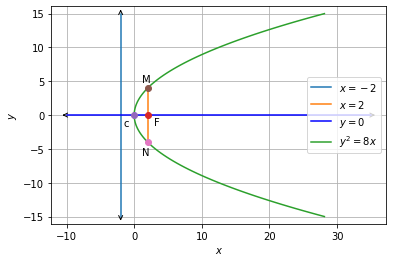
\includegraphics[width=\columnwidth]{Figure6}
\caption{Parabola $y^2=8x$ }
\label{fig:parabola}	
\end{figure}

\clearpage
\section{Generalisation}
\subsection{Circle}
\subsubsection{Property}
\begin{align}
    \vec{V}=\vec{D}=\vec{P}=\vec{I}
\end{align}
\subsubsection{Standard Form}
From \eqref{eq:veceq},
\begin{align}
    \vec{x}^T\vec{x}+2\vec{u}^T\vec{x} + f =0
\end{align}
\subsubsection{Centre}
From \eqref{eq:vertexneq},
\begin{align}
    \vec{c} = -\vec{u}
\end{align}
\subsubsection{Radius}
From \eqref{eq:stdvecneq},
\begin{align}
    \vec{r} = \sqrt{\vec{u}^T\vec{u} - f}
\end{align}
\subsection{Ellipse}
\subsubsection{Property}
\begin{align}
    \abs{\vec{V}} > 0
    \\
    \lambda_1>0,\lambda_2<0
\end{align}
\subsubsection{Standard Form}
From \eqref{eq:stdvecneq},
\begin{align}
    \frac{\vec{y}^T\vec{D}\vec{y}}{\vec{u}^T\vec{V}^{-1}\vec{u}-f}=1
\end{align}
\subsubsection{Centre}
From \eqref{eq:vertexneq},
\begin{align}
    \vec{c} = -\vec{V}^{-1}\vec{u}
\end{align}
\subsubsection{Axes}
From \eqref{eq:stdvecneq},
\begin{align}
\begin{cases}
    \sqrt{\frac{\vec{u}^T\vec{V}^{-1}\vec{u}-f}{\lambda_1}}
    \\
    \sqrt{\frac{\vec{u}^T\vec{V}^{-1}\vec{u}-f}{\lambda_2}}
\end{cases}
\end{align}
\subsection{Hyperbola}

\subsubsection{Property}
\begin{align}
    \abs{\vec{V}} < 0
    \\
    \lambda_1>0,\lambda_2<0
\end{align}
\subsubsection{Standard Form}
From \eqref{eq:stdvecneq},
\begin{align}
    \frac{\vec{y}^T\vec{D}\vec{y}}{\vec{u}^T\vec{V}^{-1}\vec{u}-f}=1
\end{align}
\subsubsection{Centre}
From \eqref{eq:vertexneq},
\begin{align}
    \vec{c} = -\vec{V}^{-1}\vec{u}
\end{align}
\subsubsection{Axes}
From \eqref{eq:stdvecneq},
\begin{align}
\begin{cases}
    \sqrt{\frac{\vec{u}^T\vec{V}^{-1}\vec{u}-f}{\lambda_1}}
    \\
    \sqrt{\frac{f-\vec{u}^T\vec{V}^{-1}\vec{u}}{\lambda_2}}
\end{cases}
\end{align}

\subsection{Parabola}
\subsubsection{Property}
\begin{align}
    \abs{\vec{V}} = 0
    \\
    \lambda_1=0
\end{align}
\subsubsection{Standard Form}
From \eqref{eq:stdveceq},
\begin{align}
    \vec{y}^T\vec{D}\vec{y} &= -2\eta\myvec{1 & 0}\vec{y} 
\end{align}
\subsubsection{Centre}
From \eqref{eq:vertex},
\begin{align}
    \myvec{\vec{u}^T + \eta\vec{p_1}^T \\ \vec{V}}\vec{c} &= \myvec{-f \\ \eta\vec{p_1} - \vec{u}} 
\end{align}
\subsubsection{Focal length}
From \eqref{eq:foclen},
\begin{align}
\beta = \frac{1}{2}\abs{\frac{\vec{u}^T\vec{p}_1}{\lambda_2}} 
\end{align}
\subsubsection{Focus}
From \eqref{eq:focus},
\begin{align}
\vec{F} = \myvec{-f \\ \eta\vec{p_1} - \vec{u}}{\myvec{\vec{u}^T + \eta\vec{p_1}^T \\ \vec{V}}}^{-1} + {\frac{-2\eta\myvec{1 & 0}}{4}}^{T} 
\end{align}
\subsubsection{Axis}
From \eqref{eq:axis},
\begin{align}
    k(\vec{V}\vec{c}+\vec{u})^{T}\vec{x} = 0 
\end{align}
\subsubsection{Directrix}
From \eqref{eq:directrix},
\begin{align}
    (\vec{V}\vec{c}+\vec{u})^T(\vec{x} +\beta) + \vec{u}^T\vec{c} + \vec{f} = 0
\end{align}
\subsubsection{Latus Rectum}
From \eqref{eq:latus},
\begin{align}
    (\vec{V}\vec{c}+\vec{u})^T(\vec{x} -\beta) + \vec{u}^T\vec{c} + \vec{f} = 0
\end{align}
\subsubsection{End points of latus rectum}
From \eqref{eq:endpt},
\begin{align}
    \vec{u}^T\kappa = -\frac{(\kappa^T\vec{V}\kappa + f )}{2}
\end{align}
\subsubsection{Length of latus rectum}
From \eqref{eq:length},
\begin{align}
   l=\norm{\beta(\vec{V}\vec{c}+\vec{u})^T} 
\end{align}

\numberwithin{table}{section}
\begin{table*}[!ht]
\begin{tabular}{ | m{1.8cm} | m{3.0cm}| m{4.0cm} | m{7.5cm} | } 
\hline
Conic  & Property & Standard Form  & Standard Parameters\\ 
\hline
Circle & $\vec{V}=\vec{D}=\vec{P}=\vec{I}$ & $\vec{x}^T\vec{x}+2\vec{u}^T\vec{x} + f =0$ & 1)Centre : $\vec{c} = -\vec{u}$ \newline 2)Radius : $ \vec{r} = \sqrt{\vec{u}^T\vec{u} - f}$  \newline \\ 
\hline
Ellipse & $\abs{\vec{V}} > 0$ \newline $\lambda_1>0,\lambda_2<0$ &   $\frac{\vec{y}^T\vec{D}\vec{y}}{\vec{u}^T\vec{V}^{-1}\vec{u}-f}=1$ & 1)Centre : $\vec{c} = -\vec{V}^{-1}\vec{u}$ \newline 2)Axes : $\begin{cases}
    \sqrt{\frac{\vec{u}^T\vec{V}^{-1}\vec{u}-f}{\lambda_1}}
    \\
    \sqrt{\frac{\vec{u}^T\vec{V}^{-1}\vec{u}-f}{\lambda_2}}\end{cases}$ \newline \\ 
\hline
Hyperbola & $\abs{\vec{V}} < 0$ \newline $\lambda_1>0,\lambda_2<0$ & $\frac{\vec{y}^T\vec{D}\vec{y}}{\vec{u}^T\vec{V}^{-1}\vec{u}-f}=1$ & 1)Centre : $\vec{c} = -\vec{V}^{-1}\vec{u}$ \newline 2)Axes : $\begin{cases}
    \sqrt{\frac{\vec{u}^T\vec{V}^{-1}\vec{u}-f}{\lambda_1}}
    \\
    \sqrt{\frac{f-\vec{u}^T\vec{V}^{-1}\vec{u}}{\lambda_2}}\end{cases}$ \newline \\
\hline
Parabola &  $\abs{\vec{V}} = 0$ \newline $\lambda_1=0$ &  $\vec{y}^T\vec{D}\vec{y} = -2\eta\myvec{1 & 0}\vec{y}$ & 1)Centre:\newline $\myvec{\vec{u}^T + \eta\vec{p_1}^T \\ \vec{V}}\vec{c} = \myvec{-f \\ \eta\vec{p_1} - \vec{u}}$ \newline 2)Focal Length: \newline $\beta = \frac{1}{2}\abs{\frac{\vec{u}^T\vec{p}_1}{\lambda_2}}$ \newline 3)Focus:\newline
$\vec{F} = \myvec{-f \\ \eta\vec{p_1} - \vec{u}}{\myvec{\vec{u}^T +$ \newline $\eta\vec{p_1}^T \\ \vec{V}}}^{-1} + {\frac{-2\eta\myvec{1 & 0}}{4}}^{T} $ \newline 4)Axis: \newline $ k(\vec{V}\vec{c}+\vec{u})^{T}\vec{x} = 0 $ \newline 5)Directrix: \newline $(\vec{V}\vec{c}+\vec{u})^T(\vec{x} +\beta) + \vec{u}^T\vec{c} + \vec{f} = 0$ \newline 6)Latus Rectum: \newline $(\vec{V}\vec{c}+\vec{u})^T(\vec{x} -\beta) + \vec{u}^T\vec{c} + \vec{f} = 0$ \newline 7)End points of latus rectum : \newline $\vec{u}^T\kappa = -\frac{(\kappa^T\vec{V}\kappa + f )}{2}$ \newline 8)Length of latus rectum: \newline $l=\norm{\beta(\vec{V}\vec{c}+\vec{u})^T}$ \newline\\
\hline
\end{tabular}
\captionsetup{justification=centering}
 \caption{Generalisation of conic}
\label{tab:table2}
\end{table*}

\end{document}
